\chapter{Quantum Computing Logic and Algorithms}

\section{Introduction}

Quantum computing uses the concepts of quantum theory to perform computations that are infeasible for classical computers. In this chapter, we will contextualise the mathematical representations introduced to understand the logic and structure of quantum computing. we will start by discussing classical computing logic and contrasting it to quantum logic. Next, we will explain the qubit, the building block of quantum computation. Then introducing quantum gates/circuits and how they manipulate quantum states. We then use Grover’s algorithm as an example algorithm to show how we can use these tools for big computational speedups, finally ending with a look at how quantum circuits can be implemented using Qiskit.
 



\section{Classical vs Quantum Logic}

\subsection{Classical Bits and Gates}

Classical computing is built on bits, a piece of data that can be in the state $0$ or $1$. These states commonly represent high or low voltages controlled by a transistor (a switch) that is either on ($1$) or off ($0$). Computations are made using logic gates, these take one or more bits as input, perform an operation on them producing an output.

\noindent The most common logic gates are:
\begin{itemize}
    \item NOT: a gate that flips the input.
    \item AND: only outputs $1$ if both inputs are $1$.
    \item OR: only outputs $1$ if one or both inputs are $1$.
    \item XOR: only outputs $1$ if the inputs are different.
\end{itemize}

\noindent These gates are represented by truth tables. For example, the AND gate truth table is:

\[
\begin{array}{c|c|c}
A & B & A \land B \\
\hline
0 & 0 & 0 \\
0 & 1 & 0 \\
1 & 0 & 0 \\
1 & 1 & 1 \\
\end{array}
\]

\noindent Classical circuits are made by combining gates to perform complex operations. An example is the half-adder, this uses an AND and XOR gate to add two bits and output a sum and a carry bit. Unlike quantum computing the logic of classical circuits is  deterministic, not probabilistic.

\noindent An important property is that classical gates are irreversible. For example, the AND gate inputs the pairs $(0,1)$, $(1,0)$, $(0,0)$ to get the same output $0$, so it's impossible to determine the inputs from just the output. Therefore, irreversibility leads to information loss, contrasted with the reversible quantum logic gates that are described by invertible linear operators (Unitary operators). Irreversibility can be seen in detail in source [27]


\subsection{Motivation for Quantum Logic}

Classical logic has several limitations. One as mentioned is:

\noindent Irreversibility: We have shown this using the example above. For each bit of lost information, according to Landauer’s principle [27], there is a thermodynamic cost (heat dissipation). Quantum Computing avoids this energy cost because of it's reversibility. 

\noindent Discreteness: Another limitation is, bits are discrete. A bit can only be one of two states, there's no way to represent superpositions of these states with classical logic. So, classical computers can't exploit or fully simulate concepts like interference or entanglements or quantum systems in general.

\noindent Quantum computing overcomes these limitations. As mentioned quantum logic gates are reversible because they're represented by unitary operators, which preserve norms and always have inverses [9]. Hence, no information is lost during computation. Furthermore, as we will show next, the qubit can live in a superposition allowing for exploitation of the above concepts.



\section{Qubits}

\subsection{The Qubit}

Similar definitions can be found in [29] and [9]. The base unit of data in quantum computing is a qubit. A qubit can exist in the state $1$, $0$ or in a superposition of both. Hence, a qubit is a quantum state represented as a vector in a two-dimensional Hilbert space:

\[
|\psi\rangle = \alpha |0\rangle + \beta |1\rangle,
\]

\noindent$|0\rangle = \begin{bmatrix}1 \\ 0\end{bmatrix}$ and $|1\rangle = \begin{bmatrix}0 \\ 1\end{bmatrix}$,is the basis, and $\alpha, \beta \in \mathbb{C}$ are the probability amplitudes satisfying the normalization condition:
\[
|\alpha|^2 + |\beta|^2 = 1.
\]

\noindent Qubits can physically be any two-level quantum system, for example energy levels in an atom.

\noindent As with any quantum system upon measurement, the qubit collapses to either $|0\rangle$ or $|1\rangle$. With the following probability given by the Born rule being:
\[
P(0) = |\alpha|^2, \quad P(1) = |\beta|^2.
\]

\noindent This measurement follows a Bernoulli distribution with a single trial, where the probability of success, for example measuring $|0\rangle$ is $p = |\alpha|^2$. Repeating the same measurement many times gives a binomial distribution of outcomes this means we can find statistical estimations of the quantum state.


\subsection{Bloch Sphere}

The Bloch sphere is an alternative graphical representation of a qubits state. Using this alternate form of a qubits state:
\[
|\psi\rangle = \cos(\theta) |0\rangle + e^{i\phi} \sin(\theta) |1\rangle,
\]

\noindent Here and as seen on figure 3.1, \( \theta \in [0, \pi] \) and \( \phi \in [0, 2\pi) \) map the qubit to a point on the surface of a unit sphere (the Bloch sphere). The angle \( \phi \) is the relative phase. It's the angle around the vertical axis of the Bloch sphere. While, \( \theta \) controls the weight of the probability amplitudes. The relative phase can distinguish between states with the same probability measurements. For example, the states \( \frac{1}{\sqrt{2}}(|0\rangle + |1\rangle) \) and \( \frac{1}{\sqrt{2}}(|0\rangle - |1\rangle) \) only differ by their relative phase. This is important as these two states behave differently in quantum circuits. The north and south poles of the Bloch sphere map to \( |0\rangle \) and \( |1\rangle \) respectively and at the equator (when \(\theta=\frac{\pi }{2}\)), are equal superpositions.



\begin{figure}[H]
    \centering
    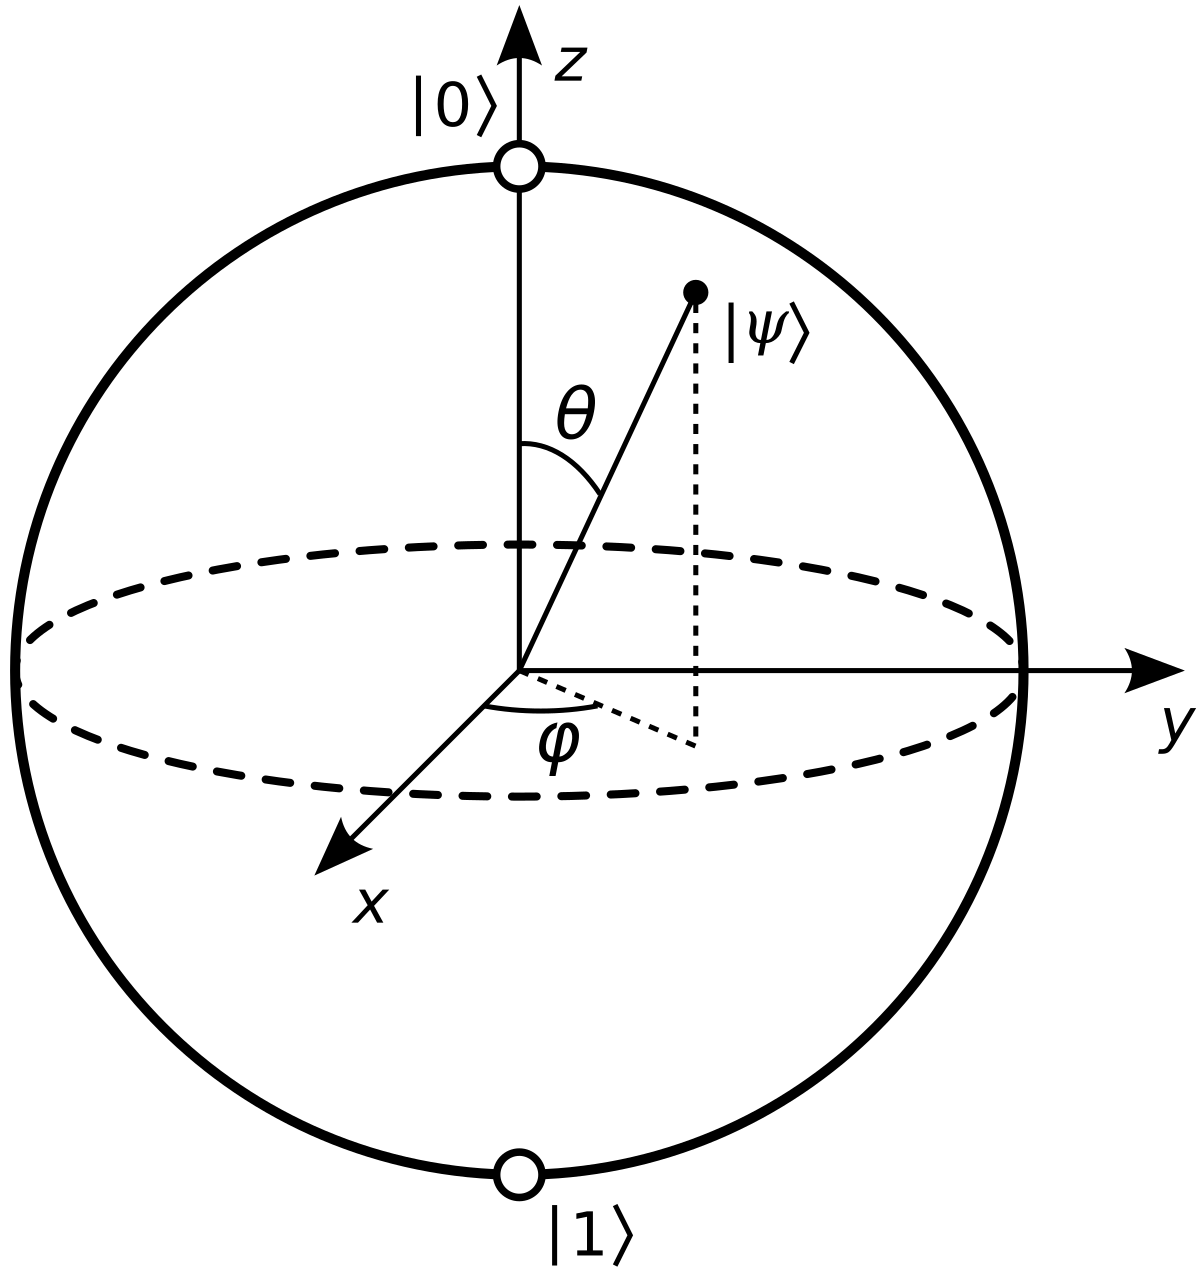
\includegraphics[width=0.4\textwidth]{Bloch_sphere.png}
    \caption{The Bloch sphere representation of a qubit, from reference [26].}
    \label{fig:bloch}
\end{figure}


\noindent The Bloch sphere is useful intuitively, as unitary transformations can be viewed as rotations about the axes. It's also useful for understanding the effects of measurement and decoherence, which collapse or shrink the qubit state towards the classical states. This section is supported by the definitions in source [9].



\subsection{Multi-Qubit State}

For  multi-qubit systems, the combined state space is the tensor product of the individual Hilbert spaces, as in section 2.6. For two qubits the joint system lives in a four-dimensional Hilbert space $\mathbb{C}^2 \otimes \mathbb{C}^2 = \mathbb{C}^4$, with the basis states:
\[
\{ |00\rangle, |01\rangle, |10\rangle, |11\rangle \}.
\]
\noindent Following from this since qubits live in a two-dimensional space we can infer that an $n$-qubit system spans a $2^n$-dimensional space as mentioned in [29]. This exponential growth in dimensions is why quantum computers can process large amounts of data in parallel as stated in [9].

\noindent The state of a multi-qubit system can be written as a superposition of these basis states. For example,  A two-qubit state is:
\[
|\psi\rangle = \alpha_{00}|00\rangle + \alpha_{01}|01\rangle + \alpha_{10}|10\rangle + \alpha_{11}|11\rangle,
\]
where $\alpha_{ij} \in \mathbb{C}$ and $\sum |\alpha_{ij}|^2 = 1$\\

\noindent In section 2.6.1 and 2.6.2 the examples we looked at for separable and entangled states were both two-qubit systems, The entangled state being the bell state [24], [25], and as we will see this is a crucial resource to quantum computers. Also we will see that quantum gates can actually generate entanglement of qubits.

\noindent It is also important to recall from Sections 2.3.4 and 2.6.3 that qubits and multi-qubit systems can be described using density matrices, both reduced and full [24],[25]. When only part of a system can be measured, reduced density matrices allow us to predict measurement outcomes, compute expectation values, and observe the local effects of quantum gates. They also help model the loss of quantum information due to entanglement with the environment, which leads to decoherence and errors in quantum systems [34].




\section{Quantum Circuits \& Gates}

\noindent Quantum circuits are made from applying multiple quantum gates to one or more qubits. As stated in Chapter 2, these unitary operators (logic gates) satisfy \( U^\dagger U = I \), this is why they're reversible and preserve probabilities until measurement.

\noindent In this section, we will define common quantum gates, for single qubits and multiple qubits, and show how they form quantum circuits. These concepts will be used later to construct algorithms and demonstrate quantum speedups.


\subsection{Single-Qubit Gates}

Single-qubit gates are applied to individual qubits to manipulate their state. As these gates are unitary operators they correspond to, $2$x$2$ complex matrices. Common single-qubit gates include:

\noindent\textbf{Pauli Gates}\\ 
\noindent The three Pauli gates, $X$, $Y$, and $Z$, are essentially 180° rotations around the $x$, $y$, and $z$ axes of the Bloch sphere [37]. They are represented by the corresponding $2$x$2$ matrices introduced in section 2.2.1.

\noindent The $X$ gate is like a classical NOT gate it flips $|0\rangle \leftrightarrow |1\rangle$, so for superpositions it switches the probability amplitudes. The $Z$ gate doesn't affect $|0\rangle$ but flips the sign of $|1\rangle$, changing the relative phase. The $Y$ gate is similar but with a complex phase. This can be backed up by [38]. \\

\noindent\textbf{The Hadamard Gate}\\
\noindent The Hadamard gate transforms the computational basis states into equal superpositions, $|+\rangle$, $|-\rangle$ and is represented by the matrix $H$:
\[
H = \frac{1}{\sqrt{2}} \begin{pmatrix} 1 & 1 \\ 1 & -1 \end{pmatrix},
\]
\[
H|0\rangle = \frac{1}{\sqrt{2}}
\begin{pmatrix}
1 & 1 \\
1 & -1
\end{pmatrix}
\begin{pmatrix}
1 \\
0
\end{pmatrix}
= \frac{1}{\sqrt{2}}
\begin{pmatrix}
1 \\
1
\end{pmatrix}
= \frac{1}{\sqrt{2}}(|0\rangle + |1\rangle)=|+\rangle,
\]

\[
H|1\rangle = \frac{1}{\sqrt{2}}
\begin{pmatrix}
1 & 1 \\
1 & -1
\end{pmatrix}
\begin{pmatrix}
0 \\
1
\end{pmatrix}
= \frac{1}{\sqrt{2}}
\begin{pmatrix}
1 \\
-1
\end{pmatrix}
= \frac{1}{\sqrt{2}}(|0\rangle - |1\rangle)=|-\rangle
\]\\
\noindent This operation moves qubits from the poles to the equator of the Bloch sphere [37], this gate creates superposition states allowing for interference.

\noindent $H$ is unitary and hermitian, so we have $H=H^\dagger$ and $H^\dagger H=HH^\dagger = I$, hence $HH=I$, this indicates that after applying the Hadamard gate, if it's applied again then the qubit states returns to the poles/are unaffected.
\\

\noindent\textbf{Phase Gates}\\
\noindent Phase gates are gates that apply phase shifts of the form $e^{\pi\varphi}$ (where $\varphi \in [0 ,2\pi]$), to just the $|1\rangle$ component of a qubit. Two common ones are the $S$ and $T$ gates:
\[
S = \begin{pmatrix} 1 & 0 \\ 0 & i \end{pmatrix}, \quad
T = \begin{pmatrix} 1 & 0 \\ 0 & e^{i\pi/4} \end{pmatrix}
\]
These gates don't affect $|0\rangle$. They rotate the qubit around the Bloch sphere’s z-axis. We can see from this that the Pauli $Z$ gate is also a phase gate. [38].



\subsection{Multi-Qubit Gates}

Multi-qubit gates are also unitary operators but they act on multiple qubits, they are used to entangle qubits. Arguably the most fundamental is the CNOT (controlled-not) gate.

\noindent The CNOT gate acts on two qubits, one is called the control the other is called the target. If the control qubits state is $|0\rangle$ then the target qubits state doesn't change. If the control qubits state is $|1\rangle$ then the target qubits state is flipped. The CNOT gate is represented by a $4$x$4$ matrix: 

\[
\text{CNOT} =
\begin{pmatrix}
1 & 0 & 0 & 0 \\
0 & 1 & 0 & 0 \\
0 & 0 & 0 & 1 \\
0 & 0 & 1 & 0
\end{pmatrix}.
\]\\
\noindent In the basis $\{|00\rangle, |01\rangle, |10\rangle, |11\rangle\}$. This gate can entangle two qubits when paired with the Hadamard gate as we will see in a later example. The CNOT gate is also well explained in [9].

\noindent Other notable multi-qubit gates include the CZ (controlled-Z) gate and the CCNOT (Toffoli) gate [29]. The CZ gate works similarly to the CNOT, it also uses a control and target qubit, if the control qubit $|0\rangle$ then the target qubits state doesn't change. But if the control qubits state is $|1\rangle$ then instead a phase shift is applied to the target qubit. The Toffoli gate is a three qubit gate that flips a target qubit if the two other qubits are both in the state $|1\rangle$ [29].


\subsection{Circuit Diagrams}

Quantum circuits are commonly represented using circuit diagrams, where the time progresses from left to right. This visual representation gives us a clear, organised way to describe sequences of gates operating on various qubits.

\noindent\textbf{Syntax} \\
\noindent Each line represents a qubit. A box with a gate name inside represents a single-qubit gate. Whereas, multi-qubit gates are shown by solid dots on the control qubits and $\oplus$ on the target qubit, connected by a vertical line. Measurement is denoted by a meter symbol or a half stadium shape with an $M$ inside. Finally, classical bits are represented by double horizontal lines. [39].

\subsubsection{Example Circuit}  
This example will show applying the Hadamard gate followed by the
CNOT gate creates an entanglement. Specifically, how the two-qubit state $|00\rangle$ becomes a Bell state:


\noindent First we apply a Hadamard gate to one of the qubits, lets say qubit one:

\[
|00\rangle \xrightarrow{H \otimes I} \frac{1}{\sqrt{2}} (|0\rangle + |1\rangle) \otimes |0\rangle
= \frac{1}{\sqrt{2}} (|00\rangle + |10\rangle),
\]

\noindent If the control is in a superposition when applying a CNOT you use the rule of the CNOT on each component of the superposition state, therefore applying the CNOT gate with qubit one as the control and two as the target:

\[
\frac{1}{\sqrt{2}} (|00\rangle + |10\rangle)\xrightarrow{\text{CNOT}} \frac{1}{\sqrt{2}} (|00\rangle + |11\rangle),
\]

\noindent This gives the entangled Bell state $|\Phi^+\rangle$ which we have seen from the examples in sections 2.6.2 and 2.6.3 is in fact entangled. We can visualise this process using this quantum circuit diagram: 
\[
\Qcircuit @C=1em @R=.7em {
& \lstick{|0\rangle} & \gate{H} & \ctrl{1} & \qw \\
& \lstick{|0\rangle} & \qw & \targ & \qw
}
\]

\noindent\textbf{Measurement in Circuits} \\
\noindent Normally at the end of a quantum circuit the qubits are measured, collapsing the states to $|0\rangle$ or $|1\rangle$ with probabilities as seen in 3.3.1. For the example bell state above, measurement over the basis $\{|00\rangle, |01\rangle, |10\rangle, |11\rangle\}$ will give the resultant states $|00\rangle$ and $|11\rangle$ with equal probabilities.

\section{Quantum Computing Algorithms}


Quantum algorithms use concepts from quantum theory to their advantage to make certain computations more efficiently than classical algorithms. Generally they start by initialising the qubits states, then a sequence of gates are applied to the qubits, and finally they are measured extracting classical results. This, as shown above, is implemented using a quantum circuits. The efficiency quantum algorithms have at specific computations is more accurately from: Superposition, namely its' ability to represent many possible inputs at once, enabling the evaluation of many inputs simultaneously. Interference, enabling quantum algorithms to steer towards the correct solution via constructive and destructive interference of probability amplitudes. Finally, entanglement, the strong correlation between qubits allows them to work together in a sense, improving the processing speed of information.


\subsection{Example Algorithm: Grover's Algorithm}
\noindent Grover’s algorithm [28] is a quantum search algorithm that's faster than typical classical search algorithms for unsorted lists. The algorithm goes as follows: 

\noindent Consider a function \( f: \{0, 1\}^n \rightarrow \{0, 1\} \) in which there is an input \( x_0 \) where \( f(x_0) = 1 \), and \( f(x) = 0 \) for all other \( x \)'s. We want to find \( x_0 \). Lets say the space the inputs live in has $ N \equiv 2^n$ items, this means $log_2(N) \equiv n$ qubits would allow the algorithm work on all possible inputs simultaneously in a superposition. This leads to the fact that while a standard classical search has an \( O(N) \) time efficiency, Grover’s algorithms is \( O(\sqrt{N}) \).\\

\noindent\textbf{Step 1 Initializing}\\
\noindent First we start all qubits in the zero state ( \( |0\rangle^{\otimes n} \)) and apply the Hadamard gate to each of them to make the system into a uniform superposition of all the possible inputs:

\[
|\psi\rangle = \frac{1}{\sqrt{N}} \sum_{x=0}^{N-1} |x\rangle.
\]\\

\noindent\textbf{Step 2: Oracle Marking}\\
\noindent An oracle \( O_f \) is then applied to the superposition state $|\psi\rangle$. The oracle is a sequence of quantum gates that flips the phase of the goal state (making its probability amplitude negative) while leaving all other states unchanged, essentially marking it. It can be written as:

\[
O_f |x\rangle = (-1)^{f(x)} |x\rangle.
\]

\noindent When applying this to $|\psi\rangle$, to mark \( |x_0\rangle \) we get:

\[
O_f |\psi\rangle = \frac{1}{\sqrt{N}} \sum_{x=0}^{N-1} (-1)^{f(x)} |x\rangle,
\]\\
\noindent\textbf{Step 3 Amplitude Amplification}\\
\noindent Next, a diffusion operator is applied to amplify the amplitude of the marked state by increasing its own amplitude and decreasing the amplitudes of all the others. This operator takes the average of the amplitudes and flips each amplitude around the average by the difference between the two. This operator is defined as:

\[
D = 2|\psi\rangle\langle\psi| - I.
\]

\noindent\textbf{Step 4 Iteration and Measurement}\\
\noindent The oracle and amplification steps by themselves don't seem very impactful but when they are iterated many times they increase the probability of the target outcome being measured immensely. A good example of how these steps work in tandem can be found in source [29] example 6.4.1. The optimal number of iterations before measurement to maximise probability of success with minimal number of iterations is $\frac{\pi}{4} \sqrt{N}
$ this is shown in source [30]. \\

\noindent\textbf{Note }Grover's algorithm is a solid example of an algorithm that uses the concepts of quantum theory namely, superposition and interference of probability amplitudes to its advantage. While, it produces a significant speedup there are other quantum algorithms like shor's that produce an exponential speedup.




\subsection{Programming on Quantum Computers}

Quantum algorithms can be made and executed using real or simulated quantum hardware. One of the most common tools for quantum programming is Qiskit, a framework modelled on python, made by IBM. Qiskit enables the construction of quantum circuits and consequently algorithms using python code, simulating their behaviour, or running them on IBM’s public quantum processors. The standard procedure of quantum programming is:
\begin{enumerate}
    \item Importing/loading Qiskit modules like \texttt{QuantumCircuit}, \texttt{Aer}, and \texttt{execute}.
    \item Initializing a quantum register (a system of qubits).
    \item Creating a sequence of gates.
    \item Adding measurement operations for extracting the resultant states of the qubits and storing them as classical information.
    \item Finally, Using a simulator or real quantum computer via the cloud to execute the program and collect the measurement results.
\end{enumerate}

\noindent One of my goals for this research project was to learn the basics of Qiskit and provide an example program that I've written. I have written a simple piece of code that demonstrates how Qiskit works and some of the key principles/fundamentals we've discussed, this can be seen in appendix B.


